\documentclass{article}

\usepackage{microtype}
\usepackage{graphicx}
\usepackage{subcaption}
\usepackage{booktabs}
\usepackage{hyperref}
\newcommand{\theHalgorithm}{\arabic{algorithm}}
\usepackage{icml2026}
\usepackage{amsmath}
\usepackage{amssymb}
\usepackage{mathtools}
\usepackage{amsthm}
\usepackage[capitalize,noabbrev]{cleveref}

\theoremstyle{plain}
\newtheorem{theorem}{Theorem}[section]
\newtheorem{proposition}[theorem]{Proposition}
\newtheorem{lemma}[theorem]{Lemma}
\newtheorem{corollary}[theorem]{Corollary}
\theoremstyle{definition}
\newtheorem{definition}[theorem]{Definition}
\newtheorem{assumption}[theorem]{Assumption}
\theoremstyle{remark}
\newtheorem{remark}[theorem]{Remark}

\icmltitlerunning{Topology-Sensitive Failure Regimes in Agentic AI}

\begin{document}

\twocolumn[
  \icmltitle{Topology-Sensitive Failure Regimes in Agentic AI:\\
  A Cross-Benchmark Trace Audit with MAS Analyzer}

  \icmlsetsymbol{equal}{*}

  \begin{icmlauthorlist}
    \icmlauthor{Anonymous Author(s)}{anon}
  \end{icmlauthorlist}

  \icmlaffiliation{anon}{Anonymous Institution}
  \icmlkeywords{agentic AI, multi-agent systems, trace diagnostics, failure modes, benchmark evaluation}

  \vskip 0.3in
]

\printAffiliationsAndNotice{}

\begin{abstract}
Multi-agent topologies are often evaluated as if additional agents were a general-purpose capability amplifier. We test that assumption with a trace-centered audit of MAS Analyzer runs across five benchmarks and seven coordination topologies. The completed corpus contains 34 benchmark--topology summary cells, 3,060 evaluated runs, 990 task-level metric rows, and 2,425 failed runs with trajectory and evaluation artifacts. The results show that topology effects are strongly benchmark-dependent: group-chat debate substantially improves StableToolBench, simple voting is strongest on BrowseComp, PlanCraft, and WorkBench, and orchestration barely moves Finance Agent despite large token costs. Trace-level failure labels reveal why: benchmark identity largely determines the dominant failure regime, while topology mostly changes cost, communication, and the probability of escaping that regime. We argue that agent evaluation should report topology-sensitive failure regimes and coordination tax, not only terminal success.
\end{abstract}

\section{Introduction}
Agentic systems are increasingly evaluated through benchmark success rates, but terminal scores hide the process by which a run fails. A final answer can be wrong because retrieval locked onto a weak hypothesis, because a planner declared impossibility after a local shortage, because an API returned sparse evidence, or because a workflow never grounded a required person or email address. These are not interchangeable errors: each implies a different repair.

This paper studies whether multi-agent topology changes those failures. The question is deliberately narrower than ``do more agents help?'' We ask when topology changes success, when it only changes cost, and when the same benchmark-specific failure regime persists across coordination structures. We analyze a MAS Analyzer experiment suite spanning \textit{browsecomp}, \textit{plancraft}, \textit{stabletoolbench}, \textit{workbench}, and \textit{finance\_agent}. The evaluated systems include a single-agent baseline, flat voting, fully linked debate, group-chat debate, and three orchestrator variants.

Our central finding is that topology is not a universal intervention. The strongest topology differs by benchmark, and the largest success gain appears only on the tool-heavy StableToolBench. On several other benchmarks, richer coordination adds substantial token and communication overhead while leaving the dominant failure mode largely intact. We therefore frame failure modes as topology-sensitive but benchmark-anchored: topology can change the chance of escaping a failure regime, but the regime itself is usually induced by the benchmark's evidence and action structure.

The paper makes three contributions. First, it reports a cross-benchmark topology matrix over 34 completed benchmark--topology cells. Second, it codes 2,425 failed runs into operational failure regimes using evaluation JSON, trajectory markdown, and representative trace inspection. Third, it introduces a coordination-tax view that relates success lift to token and communication overhead, making expensive multi-agent gains easier to interpret.

\section{Related Work}
Our study builds on agent architectures that interleave reasoning, action, tool use, and feedback. ReAct showed how reasoning traces can be coupled with environment interaction \cite{react}; Toolformer studied learned tool invocation \cite{toolformer}; Reflexion emphasized verbal feedback after failed attempts \cite{reflexion}; and AutoGen made multi-agent conversation a practical systems pattern \cite{autogen}. These works motivate the topologies we study, but they do not determine when coordination repairs failures rather than amplifying them.

Benchmark work has likewise exposed the brittleness of long-horizon execution. AgentBench evaluates LLMs as agents across interactive settings \cite{agentbench}, and WebArena shows that realistic web tasks create failures not captured by static question answering \cite{webarena}. Our contribution is complementary: rather than introduce a new benchmark, we use a common artifact format to compare how benchmark families interact with topology.

The distinction matters because many benchmark reports emphasize issue-level trends in final correctness. Our traces show that long-horizon drift often begins earlier: an evidence state becomes thin, a tool response becomes a bottleneck, or a grounded entity remains unresolved. Reflection and debate are useful only if they detect that boundary. When every agent inherits the same weak context, multi-agent discussion can become redundant confirmation rather than adversarial verification.

\section{Corpus and Method}
\subsection{Experiment Scope}
The suite contains five benchmarks and seven topology labels: \texttt{sas}, \texttt{only\_voting}, \texttt{fully\_linked\_debate}, \texttt{group\_chat\_debate}, \texttt{orchestrator\_no\_discussion}, \texttt{orchestrator\_tree\_structure}, and \texttt{orchestrator\_with\_discussion}. One aggregate summary cell is absent from the completed export, leaving 34 benchmark--topology cells. Each completed cell has 30 tasks and three repeated runs, yielding 3,060 evaluated runs. The task-level metric export contains 990 task rows over 33 cells and is used for token, latency, communication, handoff, and tool-call analysis.

\begin{figure*}[t]
\centering
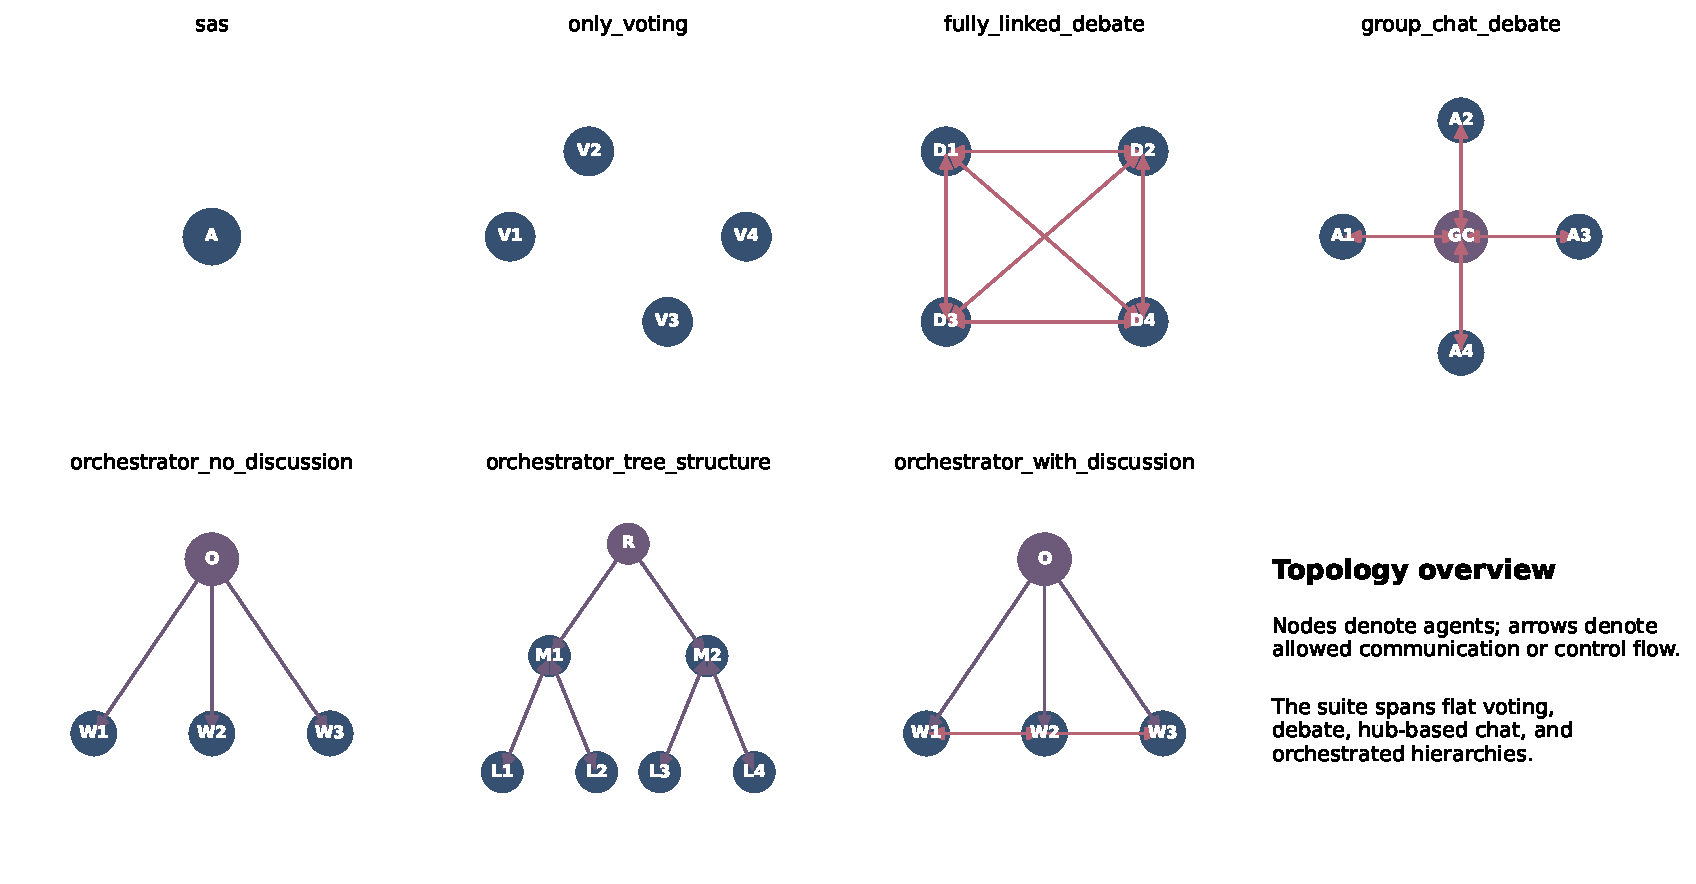
\includegraphics[width=0.95\textwidth]{figures/topology_overview.pdf}
\caption{The evaluated topologies span single-agent execution, independent voting, connected debate, group chat, and orchestrated control.}
\label{fig:topology_overview}
\end{figure*}

\subsection{Metrics}
We report task success, stability across repeated runs, average token use, tool calls, communication count, and handoff count. For topology comparisons, we compute success lift relative to \texttt{sas} within the same benchmark and token multiplier relative to the same baseline. This gives a direct estimate of coordination tax: the extra inference budget spent for each topology-specific success gain.

\subsection{Failure Coding}
We code every failed run in the 34 completed cells, for 2,425 failures in total. Coding begins from the benchmark evaluator output, then uses the prediction string, final reason, trajectory markdown, and representative JSONL traces to assign one primary label. The labels are operational rather than universal. For example, PlanCraft failures are coded as \emph{premature impossibility} when the run emits \texttt{impossible} after a local shortage; WorkBench failures are coded as \emph{entity grounding failure} when a missing person, sender, email, or assignee blocks execution.

This is a lightweight trace audit, not a multi-rater annotation study. Its purpose is diagnostic: to identify whether failures across topologies share the same trace-visible mechanism, and whether topology changes the distribution of those mechanisms.

\section{Topology Does Not Have a Universal Winner}
\begin{figure*}[t]
\centering
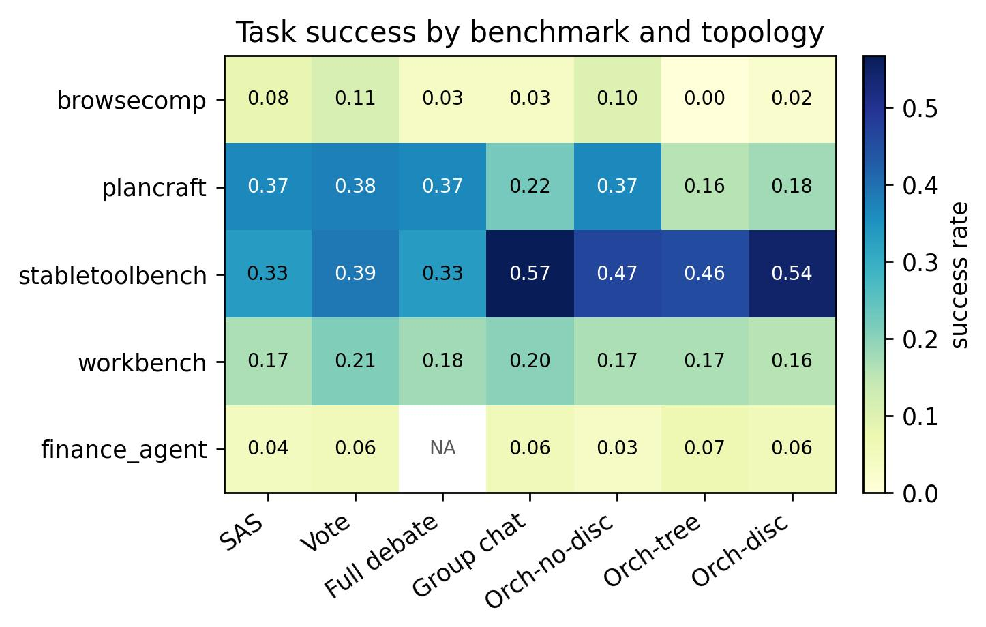
\includegraphics[width=0.95\textwidth]{figures/topology_success_heatmap.pdf}
\caption{Task success by benchmark and topology. No topology dominates across benchmarks; topology effects are largest on StableToolBench and weakest on Finance Agent.}
\label{fig:success_heatmap}
\end{figure*}

\cref{fig:success_heatmap} shows the central result. \texttt{only\_voting} is strongest on BrowseComp, PlanCraft, and WorkBench; \texttt{group\_chat\_debate} is strongest on StableToolBench; and \texttt{orchestrator\_tree\_structure} is strongest on Finance Agent. The best topology is therefore benchmark-dependent, not a general property of agent count.

\begin{table}[t]
\centering
\small
\resizebox{\columnwidth}{!}{%
\begin{tabular}{l l c c c c}
\toprule
Benchmark & Best topology & Best & SAS & Lift & Token mult. \\
\midrule
browsecomp & only\_voting & .111 & .078 & +.033 & 4.3$\times$ \\
plancraft & only\_voting & .378 & .367 & +.011 & 3.9$\times$ \\
stabletoolbench & group\_chat\_debate & .567 & .333 & +.233 & 9.7$\times$ \\
workbench & only\_voting & .211 & .167 & +.044 & 3.5$\times$ \\
finance\_agent & orchestrator\_tree\_structure & .067 & .044 & +.022 & 8.4$\times$ \\
\bottomrule
\end{tabular}}
\caption{Best topology by benchmark. The largest gain appears on StableToolBench, but it also requires the largest token multiplier among the winners.}
\label{tab:best}
\end{table}

\cref{tab:best} makes the trade-off explicit. StableToolBench gains 23.3 points over \texttt{sas}, while PlanCraft gains only 1.1 points despite using nearly four times as many tokens. Finance Agent is even more sobering: the best topology uses 8.4$\times$ the baseline tokens for a 2.2-point success lift. These results already suggest that coordination is useful only when it matches the benchmark's bottleneck.

\begin{figure*}[t]
\centering
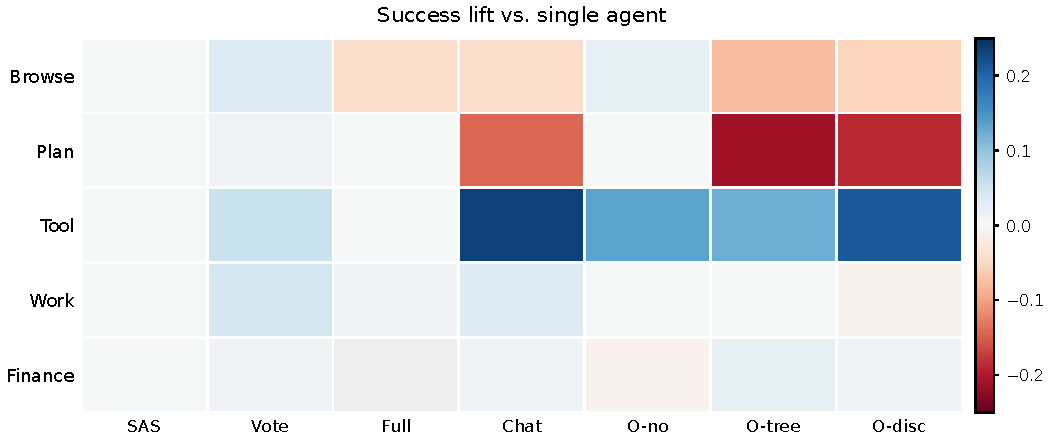
\includegraphics[width=0.95\textwidth]{figures/topology_delta_heatmap.pdf}
\caption{Success lift relative to \texttt{sas}. Positive effects concentrate in StableToolBench; several debate and orchestrator variants underperform the single-agent baseline on BrowseComp and PlanCraft.}
\label{fig:delta_heatmap}
\end{figure*}

\section{Failure Regimes Are Benchmark-Anchored}
\begin{figure}[t]
\centering
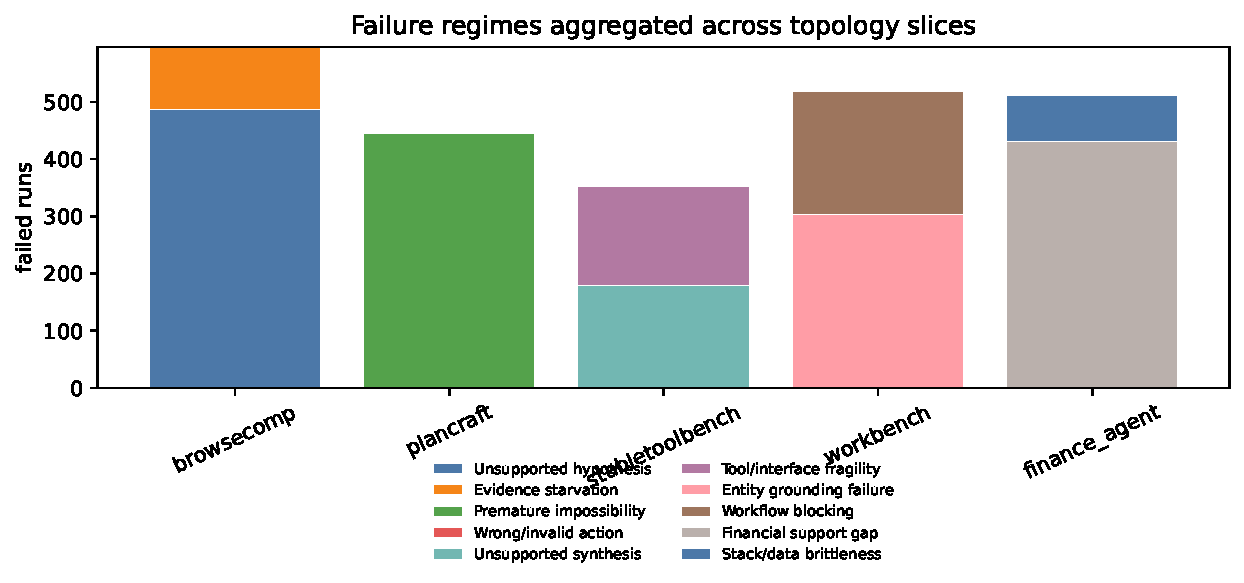
\includegraphics[width=\columnwidth]{figures/failure_regimes_all_topologies.pdf}
\caption{Failure labels aggregated across completed topology slices. The dominant failure regime is largely determined by benchmark family.}
\label{fig:failure_regimes}
\end{figure}

\cref{fig:failure_regimes} aggregates all failed runs in completed cells. BrowseComp is dominated by unsupported hypotheses: 487 of 596 failed runs return an answer whose support chain is too weak, while 109 explicitly report evidence starvation. PlanCraft is the cleanest regime: 444 of 447 failures are premature impossibility. StableToolBench splits between unsupported synthesis (180) and tool/interface fragility (172), showing that tool-heavy tasks fail both at the interface and at the synthesis layer. WorkBench failures are mostly grounding related: 304 entity grounding failures and 214 broader workflow blocks. Finance Agent is dominated by financial support gaps (430 of 512), with 82 stack or data brittleness cases.

The important point is not that these labels are perfect. The important point is that topology rarely erases the benchmark's dominant regime. In BrowseComp, several coordination-heavy systems spend many more tokens but still fail by building around weak evidence. In PlanCraft, debate and orchestration do not prevent the local-to-global impossibility jump. In WorkBench, additional agents cannot execute a workflow if none of them resolves the missing entity. StableToolBench is the main exception: because its bottleneck often involves assembling partial tool evidence, group discussion can actually change the run's chance of success.

\section{Topology Changes Cost Before It Changes Failure}
\begin{figure}[t]
\centering
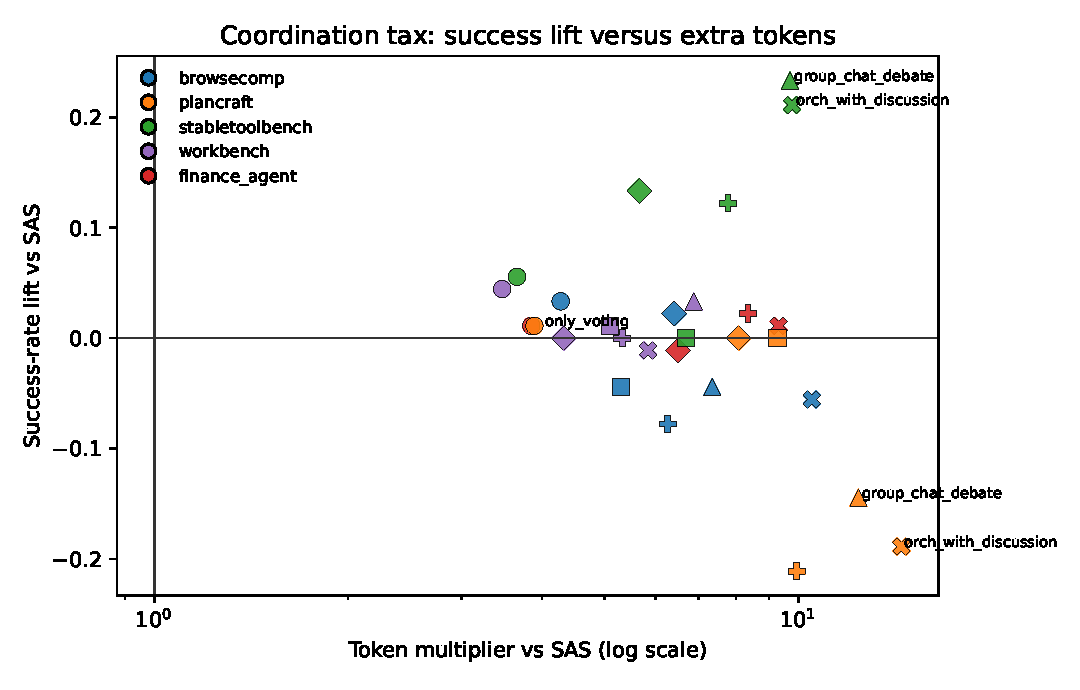
\includegraphics[width=\columnwidth]{figures/coordination_tax_plane.pdf}
\caption{Coordination tax: success lift versus token multiplier relative to \texttt{sas}. StableToolBench is the only clear high-cost, high-gain case.}
\label{fig:coordination_tax}
\end{figure}

\cref{fig:coordination_tax} plots the economic side of the same story. Across non-\texttt{sas} topologies, \texttt{only\_voting} has the highest mean success lift (+3.1 points) with a lower mean token multiplier than discussion-heavy systems. \texttt{group\_chat\_debate} has high variance: it is excellent on StableToolBench but weak on BrowseComp and PlanCraft. \texttt{orchestrator\_with\_discussion} is especially costly, with negative mean lift across the task-level metric export.

This suggests a practical diagnostic: evaluate whether extra coordination changes the evidence state. If additional agents introduce genuinely new tool evidence or independent checks, the tax may be justified. If they merely paraphrase the same weak intermediate claim, the system pays for redundancy. The failure traces repeatedly show the latter pattern in BrowseComp and PlanCraft: discussion increases commitment or deliberation length without changing the decisive state variable.

\section{Clinical Trace Anatomy}
\subsection{BrowseComp: Hypothesis Lock-In}
In a representative BrowseComp failure, the system must identify the correct institution associated with a target entity. Early retrieval returns partial matches near a plausible candidate. A voting or discussion topology then promotes that candidate into the working hypothesis. Subsequent queries become refinements around the same institution rather than tests of whether the institution is actually supported.

The fatal pivot is the moment a provisional lead becomes the organizing context. From that point onward, later turns are locally coherent but globally narrowing. Multi-agent discussion does not repair the run because every agent is reasoning over nearly the same thin evidence slice. The missing mechanism is adversarial evidence testing: a requirement that a candidate survive disconfirming retrieval, not merely repeated mention.

\subsection{PlanCraft: Local Shortage Becomes Global Impossibility}
In a representative PlanCraft failure, the agent correctly parses the target and inventory but encounters a missing intermediate resource. The correct next question is whether an alternate recipe, smelting step, or transformation route can produce the missing item. Instead, the run emits \texttt{impossible}. One concrete trajectory for pink dye states that red dye is absent even though the inventory contains a poppy that could support the route.

The failure is not a lack of domain language. It is a state-transition error: ``current branch blocked'' is converted into ``goal impossible.'' More agents help only if one agent explicitly preserves the unexplored frontier. Otherwise, coordination gives the same mistaken transition more surface area.

\section{Toward Mechanistic Evaluation}
The audit supports a state-space view of agentic failure. Each retrieval, tool call, or entity lookup updates the latent execution state. A later action may look reasonable while inheriting a corrupted state. BrowseComp failures often inherit a narrowed hypothesis space; PlanCraft failures inherit an invalid impossibility state; WorkBench failures inherit an unresolved entity binding; StableToolBench failures inherit a low-information tool state.

This framing turns failure labels into falsifiable mechanistic hypotheses. If evidence starvation is the driver, then forcing diverse retrieval or measuring unique evidence growth should change outcomes. If premature impossibility is the driver, then a formal frontier-exhaustion check should reduce false \texttt{impossible} actions. If tool fragility is the driver, causal interventions on tool responses should shift unsupported synthesis rates. The value of traces is that these hypotheses can be tested at the state-transition level, not only at the final-answer level.

\section{Implications for System Design}
The results argue against topology selection by leaderboard average alone. A useful multi-agent system should match coordination to failure regime. Tool-heavy tasks benefit from discussion when agents can combine partial external evidence. Search tasks need stagnation detection and adversarial evidence checks. Planning tasks need formal impossibility standards. Workflow tasks need early entity grounding before deeper orchestration. Finance tasks need support-sensitive answer policies that penalize fluent unsupported specificity.

The evaluation protocol should also report coordination tax. A topology that gains one or two points at 8--10$\times$ token cost may be valuable in a high-stakes setting, but it should not be reported as an unqualified improvement. Conversely, a cheap topology with modest gains may be a better default when the dominant failure mode is not repaired by discussion.

\section{Threats to Validity}
This study analyzes one experiment batch and one model family. The topology effects may change with stronger models, better tool interfaces, or different prompts. The failure labels are primary labels; many runs exhibit mixed mechanisms, especially tool fragility followed by unsupported synthesis. The coding procedure combines programmatic filtering with trace inspection rather than independent multi-rater annotation. Finally, one aggregate topology cell is absent from the completed summary export, so cost and task-level metric comparisons use the available completed cells.

\section{Conclusion}
Across five benchmarks and seven topology labels, multi-agent coordination is not a universal fix for agentic failure. StableToolBench benefits substantially from group-chat debate, but BrowseComp, PlanCraft, WorkBench, and Finance Agent show much smaller gains or expensive stagnation. The trace audit explains why: benchmark family largely determines the dominant failure regime, while topology mainly changes the cost and probability of escaping it. Future agent evaluation should therefore report topology-sensitive failure regimes, state-transition diagnostics, and coordination tax alongside terminal success.

\section*{Impact Statement}
This paper studies failure in agentic AI systems with the goal of improving reliability and transparency. The positive impact is methodological: trace diagnostics can help developers separate unsupported answers from well-supported ones, distinguish tool failures from reasoning failures, and choose coordination structures with clearer evidence. The risk is that failure triggers could be used to construct adversarial tasks or to overfit systems to benchmark artifacts. In finance-style settings, fluent numerical answers with weak support chains are especially concerning because they can appear credible while failing a faithfulness test. We therefore recommend reporting failure taxonomies together with benchmark scope, uncertainty, and the limits of each diagnosis.

\bibliography{example_paper}
\bibliographystyle{icml2026}

\newpage
\appendix
\onecolumn

\section{Failure Coding Rubric}
\begin{itemize}
    \item \textbf{Unsupported hypothesis}: the run returns a candidate answer without sufficient supporting evidence.
    \item \textbf{Evidence starvation}: the run explicitly reports that necessary evidence was not recovered.
    \item \textbf{Premature impossibility}: the run emits \texttt{impossible} before the search frontier is exhausted.
    \item \textbf{Tool/interface fragility}: sparse, empty, inconsistent, or unavailable tool output is the primary bottleneck.
    \item \textbf{Unsupported synthesis}: tools return some evidence, but the final answer exceeds what the evidence supports.
    \item \textbf{Entity grounding failure}: a person, email, sender, recipient, user, or assignee cannot be resolved.
    \item \textbf{Workflow blocking}: execution stalls on an operational precondition not captured by entity grounding alone.
    \item \textbf{Financial support gap}: a financial answer is fluent or numerically specific but weakly supported.
    \item \textbf{Stack/data brittleness}: finance failures caused by interacting data, interface, and benchmark constraints.
\end{itemize}

\section{Reproducible Trigger Metrics}
\begin{table}[h]
\centering
\small
\begin{tabular}{p{0.30\textwidth} p{0.31\textwidth} p{0.30\textwidth}}
\toprule
Trigger & Diagnostic metric & Expected failure regime \\
\midrule
Repeated search with overlapping snippets & Unique-document growth across retrieval turns & Evidence starvation or unsupported hypothesis \\
Early \texttt{impossible} after a local shortage & Alternate route expansions before termination & Premature impossibility \\
Repeated sparse tool outputs & Low-information response streak length & Tool/interface fragility \\
Missing person or email before first action & Unresolved binding count & Entity grounding failure \\
Specific numerical answer with thin support & Support density and source disagreement & Financial support gap \\
\bottomrule
\end{tabular}
\caption{Trace-local triggers that can be converted into programmatic assertions.}
\label{tab:triggers}
\end{table}

\section{Artifact Notes}
The primary aggregate file is \texttt{experiment\_summary.csv}. Task-level metrics are drawn from \texttt{Plot/system\_level\_metrics.csv} and \texttt{Plot/task\_level\_metrics.csv}. Per-run diagnoses use \texttt{run\_*.eval.json}, \texttt{run\_*.trajectory.md}, and \texttt{run\_*.trace.jsonl}. The analysis excludes incomplete aggregate cells from topology-level summary claims.

\end{document}
